%!TEX TS-program = xelatex 
%!TEX encoding = UTF-8 Unicode 

\documentclass[fontsize=11pt, paper=a4, 
DIV15,
headings=normal,
parskip=half-, 
numbers=noenddot]{scrartcl}

\usepackage[british]{babel} 

\usepackage{fontspec,xltxtra,xunicode} 
\defaultfontfeatures{Mapping=tex-text} 

\setromanfont[Mapping=tex-text]{DejaVu Serif}
\setsansfont[Scale=MatchLowercase,Mapping=tex-text]{Helvetica} 
\setmonofont[Scale=1.0]{Courier New} 

\frenchspacing

\usepackage{graphicx}
\graphicspath{{../../Bilder/}}

\usepackage{longtable}

\usepackage{philokalia}

\usepackage{yfonts}
\usepackage{rotunda}

%%%

\input{../../abbreviations/abbreviations_2}

\begin{document}

\begin{center}
{\fontspec{Helvetica}{\LARGE \textbf{
Special Instructions for Heytesbury (1494)\\[3mm]
(Addendum to Data Entry Specs 2.0) 
}}} \\[5mm]
\large Wolfgang Schmidle, Paul Trzeciok, Klaus Thoden, Malcolm D. Hyman

\normalsize Max Planck Institute for the History of Science, Berlin, Germany

\today
\end{center}


The following sections of the Data Entry Specs 2.0 are relevant: ...


\section{The Characters}

The font in Heytesbury resembles the font given in the following table.

%\vspace{2mm}
%\begin{tabelle}[: \, Breitkopf Fraktur (Walden)]
%\begin{tabular}{@{}lc@{ }c@{ }c@{ }c@{ }c@{ }c@{ }c@{ }c@{ }c@{ }c@{ }c@{ }c@{ }c@{ }c@{ }c@{ }c@{ }c@{ }c@{ }c@{ }c@{ }c@{ }c@{ }c@{ }c@{ }c@{ }c} \\
%small letters & \fraktur{a} & \fraktur{b} & \fraktur{c} & \fraktur{d} & \fraktur{e} & \fraktur{f} & \fraktur{g} & \fraktur{h} & \fraktur{i} & \fraktur{j} & \fraktur{k} & \fraktur{l} & \fraktur{m} & \fraktur{n} & \fraktur{o} & \fraktur{p} & \fraktur{q} & \fraktur{r} & \fraktur{s <} & \fraktur{t} & \fraktur{u} & \fraktur{v} & \fraktur{w} & \fraktur{x} & \fraktur{y} & \fraktur{z} \\[2mm]
% & §a§ & §b§ & §c§ & §d§ & §e§ & §f§ & §g§ & §h§ & §i§ & §j§ & §k§ & §l§ & §m§ & §n§ & §o§ & §p§ & §q§ & §r§ & §$§ §s§ & §t§ & §u§ & §v§ & §w§ & §x§ & §y§ & §z§ \\ 
% \\ 
%capital letters & \fraktur{A} & \fraktur{B} & \fraktur{C} & \fraktur{D} & \fraktur{E} & \fraktur{F} & \fraktur{G} & \fraktur{H} & \fraktur{I} && \fraktur{K} & \fraktur{L} & \fraktur{M} & \fraktur{N} & \fraktur{O} & \fraktur{P} & \fraktur{Q} & \fraktur{R} & \fraktur{S} & \fraktur{T} & \fraktur{U} & \fraktur{V} & \fraktur{W} & \fraktur{X} & \fraktur{Y} & \fraktur{Z} \\[2mm]
% & §A§ & §B§ & §C§ & §D§ & §E§ & §F§ & §G§ & §H§ & §I§ && §K§ & §L§ & §M§ & §N§ & §O§ & §P§ & §Q§ & §R§ & §S§ & §T§ & §U§ & §V§ & §W§ & §X§ & §Y§ & §Z§ \\ 
% \\ 
%\end{tabular}
%\end{tabelle}

\vspace{2mm}
\begin{tabelle}[: \, gothic alphabet]
\begin{tabular}{@{}lc@{ }c@{ }c@{ }c@{ }c@{ }c@{ }c@{ }c@{ }c@{ }c@{ }c@{ }c@{ }c@{ }c@{ }c@{ }c@{ }c@{ }c@{ }c@{ }c@{ }c@{ }c@{ }c@{ }c@{ }c@{ }c} \\
small letters & \textgoth{a} & \textgoth{b} & \textgoth{c} & \textgoth{d} & \textgoth{e} & \textgoth{f} & \textgoth{g} & \textgoth{h} & \textgoth{i} & \textgoth{j} & \textgoth{k} & \textgoth{l} & \textgoth{m} & \textgoth{n} & \textgoth{o} & \textgoth{p} & \textgoth{q} & \textgoth{r} & \textgoth{s s:} & \textgoth{t} & \textgoth{u} & \textgoth{v} & \textgoth{w} & \textgoth{x} & \textgoth{y} & \textgoth{z} \\[2mm]
 & §a§ & §b§ & §c§ & §d§ & §e§ & §f§ & §g§ & §h§ & §i§ & §j§ & §k§ & §l§ & §m§ & §n§ & §o§ & §p§ & §q§ & §r§ & §$§\,§s§ & §t§ & §u§ & §v§ & §w§ & §x§ & §y§ & §z§ \\ 
 \\ 
capital letters & \textgoth{A} & \textgoth{B} & \textgoth{C} & \textgoth{D} & \textgoth{E} & \textgoth{F} & \textgoth{G} & \textgoth{H} & \textgoth{I} && \textgoth{K} & \textgoth{L} & \textgoth{M} & \textgoth{N} & \textgoth{O} & \textgoth{P} & \textgoth{Q} & \textgoth{R} & \textgoth{S} & \textgoth{T} & \textgoth{U} & \textgoth{V} & \textgoth{W} & \textgoth{X} & \textgoth{Y} & \textgoth{Z} \\[2mm]
 & §A§ & §B§ & §C§ & §D§ & §E§ & §F§ & §G§ & §H§ & §I§ && §K§ & §L§ & §M§ & §N§ & §O§ & §P§ & §Q§ & §R§ & §S§ & §T§ & §U§ & §V§ & §W§ & §X§ & §Y§ & §Z§ \\ 
 \\ 
\end{tabular}
\end{tabelle}

(Buchstaben, die nicht vorkommen, weglassen! k, v?)

\textgoth{! " \# \$ \%}

(Fraktur-Kapitel durchgehen! z.B. Standard-Ligaturen nicht markieren)

eher Rotunda als Fraktur? Nur das Q sieht ähnlich aus.

Please type the “alternative r” as normal §r§.

Please make sure to distinguish between these pairs of similar characters:

 §b§ and §h§; §r§ and §x§; §f§ and §s§, §i§ and §\.r§

\textgoth{b} and \textgoth{h} (§b§ and §h§),
\textgoth{r} and \textgoth{x} (§r§ and §x§),
\textgoth{f} and \textgoth{s} (§f§ and §$§), 
\textgoth{i} and \textgoth{...} (§i§ and §\.r§)


\begin{mainrule}
\end{mainrule}

\begin{clarification}
\end{clarification}

\begin{note}
\end{note}

doch §3§ für §{et}§? Oder als §z§ tippen lassen, weil es keine echten z gibt? Ligatur §$z§ (sed) als Ligatur markieren lassen? Eigentlich nicht nötig, denn es ist eine bekannte Abkürzung.

Enthält der Text Zahlen (außer Seitenzahlen)?

auch einen Code für "hochgestellte 9"


allgemein: einfache Buchstaben, oder Klammer-Notation?

\begin{example}[ 2: \, bla bla]

%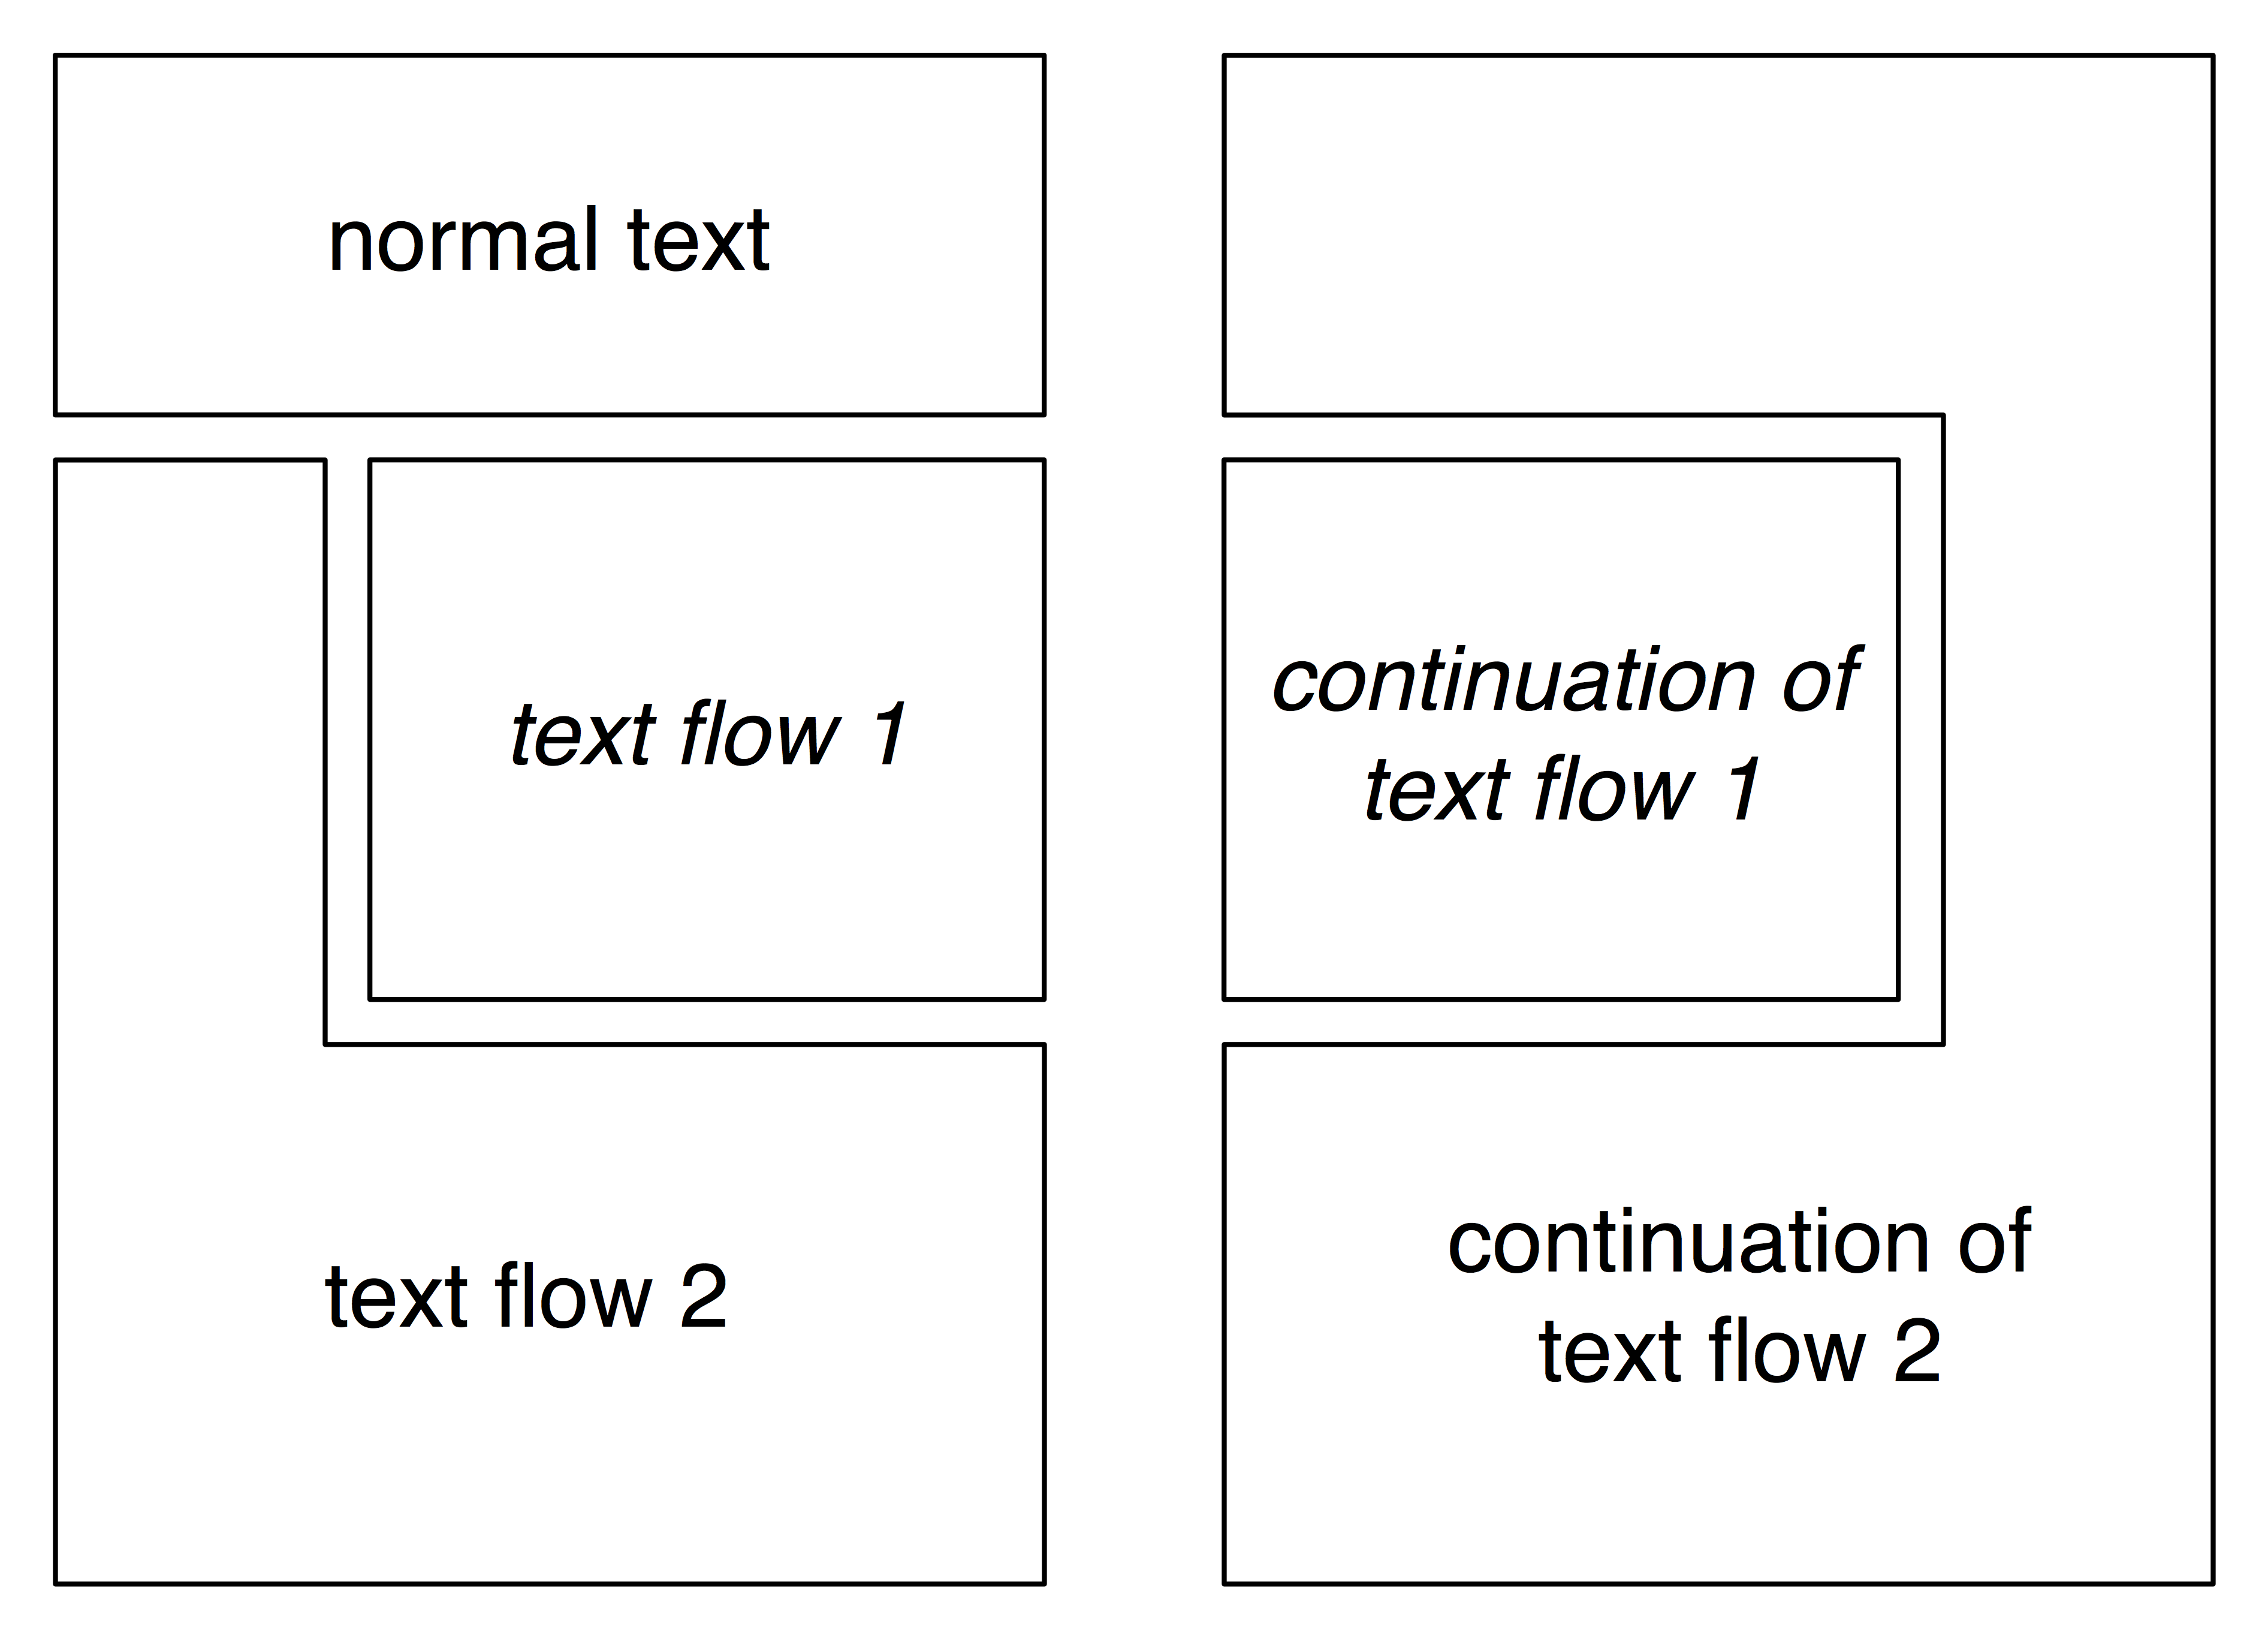
\includegraphics[width=12cm]{two_textflows.pdf}

\begin{typeLatin}
\end{typeLatin}
\end{example}

\section{Large Font}

\begin{mainrule}
Mark large font by §<lg> </lg>§. Mark indented text as headings, i.e. §<h> </h>§.
\end{mainrule}

\vspace{3mm}
\begin{sampleImage}[: \, p.014]{Heytesbury-014-linksoben}

\begin{typeLatin}
\bold{<pb><rh>}De $cire\bold{</rh>} \\
\bold{<col 1>} \\
\bold{<h>}¶ De $cire \li{et} dubitare.\bold{</h>} \\
\bold{<p><lg>}SCire multis\bold{</lg>} modis d\bs.r: $z $iue \\

dica\bs~t \li{pro}\bs.pe $iue c\\\


$truant\li{ur}   ornat\li{us}    \bs~itercurrunt \\

\bold{<pb>} \\
normal text \\
\bold{<tf 1 it>} \\
text flow 1 \\
\bold{</tf>} \\
\bold{<tf 2>} \\
text flow 2 \\
\bold{</tf>} \\ \\
\bold{<pb>} \\
\bold{<tf 1 it>} \\
continuation of \\ 
text flow 1 \\
\bold{</tf>} \\
\bold{<tf 2>} \\
continuation of \\ 
text flow 2 \\
\bold{</tf>} \\
\end{typeLatin}
\end{sampleImage}


\end{document}
